
\begin{figure}
	\begin{center}
		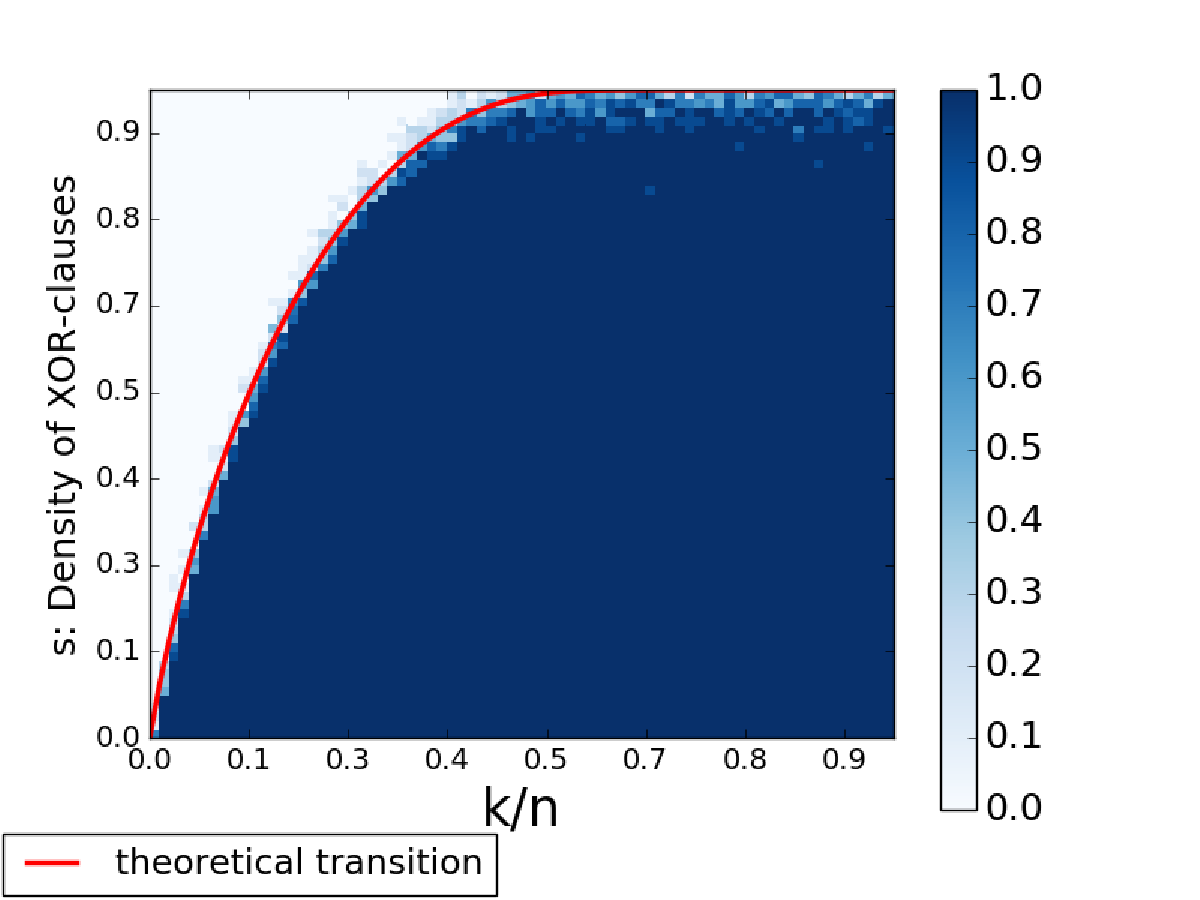
\includegraphics[width= 1\columnwidth]{pb-experiments/satisfiability/add/75boundary.pdf}
	\end{center}
	\caption{This plot shows the satisfiability behavior for $n=75$. The darker shade of blue indicates the instances which were satisfiable with higher probability and the red line shows the theoretically derived phase transition. (Best viewed in color)} 
	\label{fig:satisfiablitiy}
\end{figure}
\begin{figure*}
	\begin{multicols}{3}
		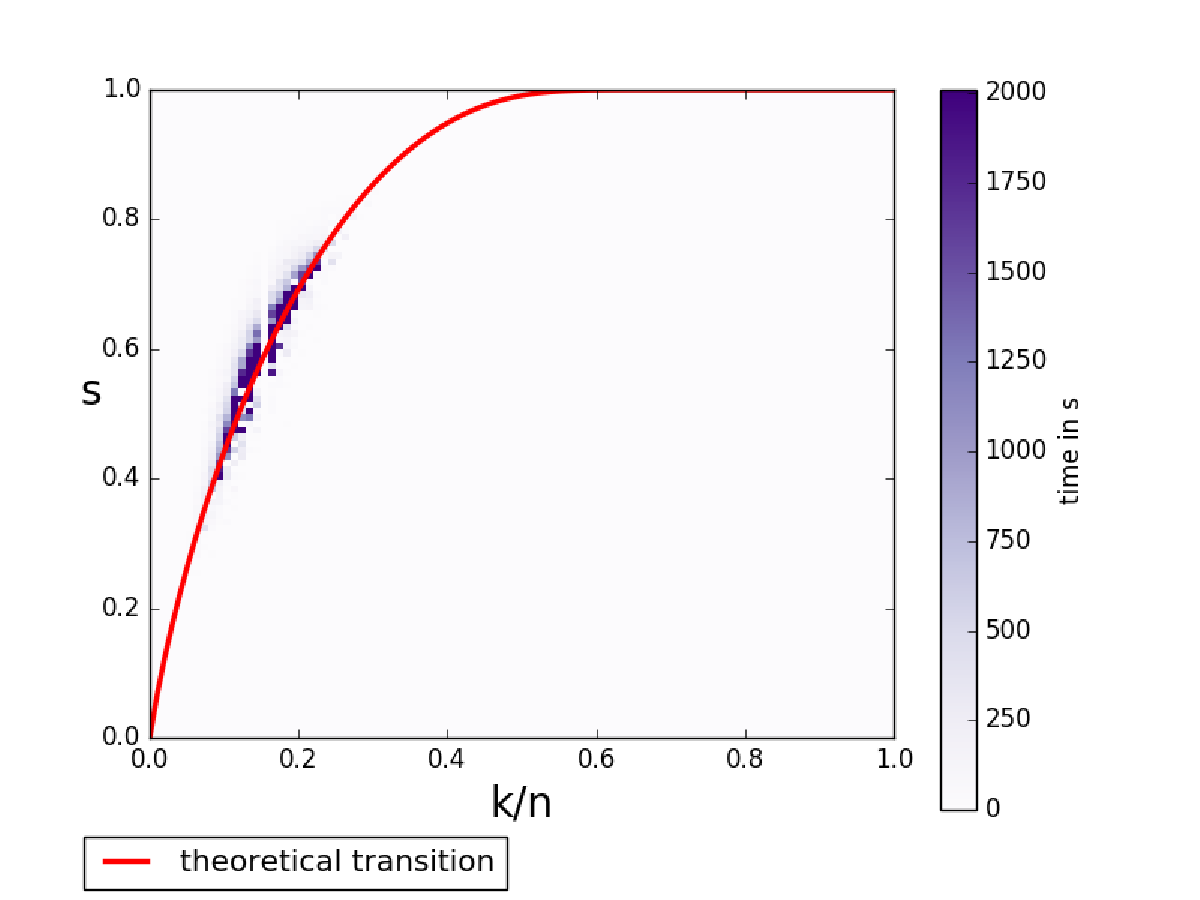
\includegraphics[width=1\linewidth]{pb-experiments/runtime/card/100.pdf}\par
		\captionof{figure}*{$n=100$}
		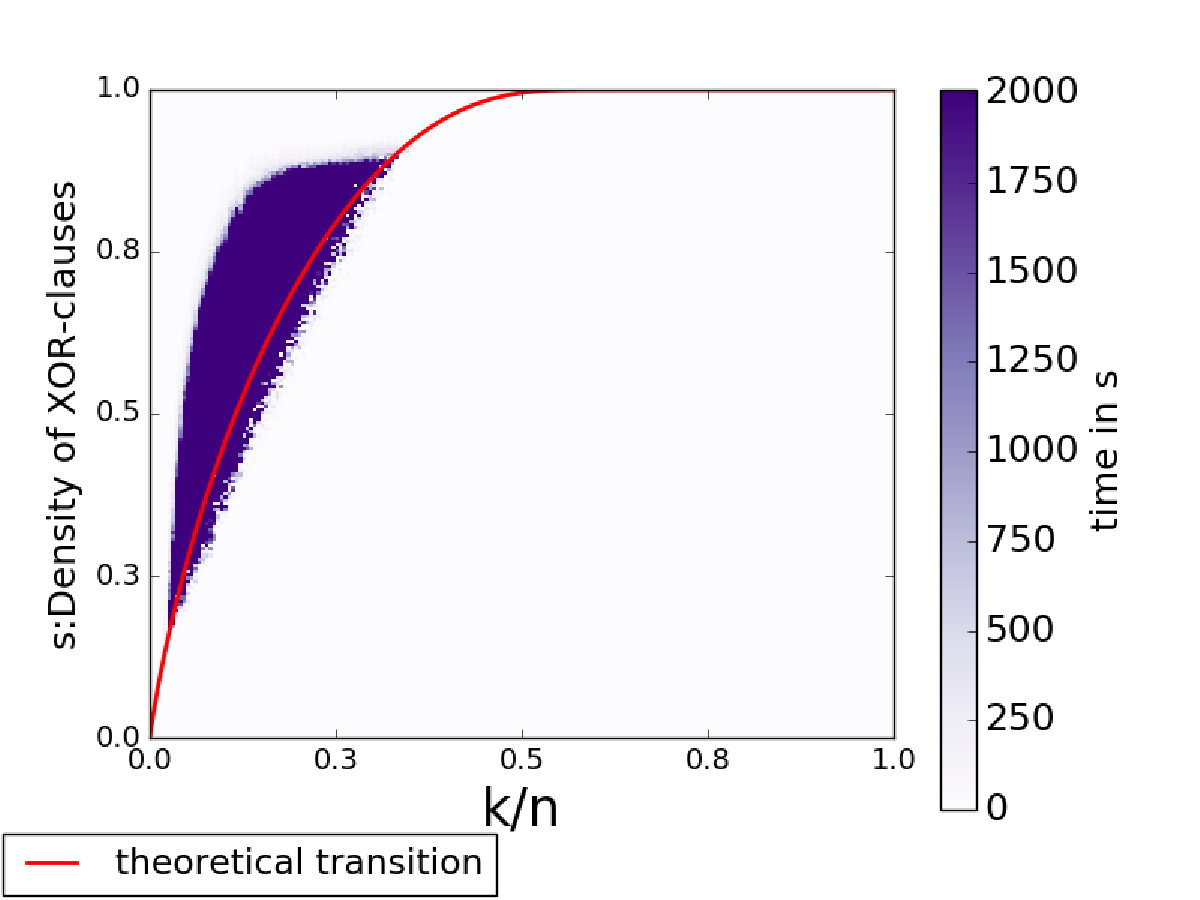
\includegraphics[width=1\linewidth]{pb-experiments/runtime/card/200.pdf}\par 
		\captionof{figure}*{$n=200$}
		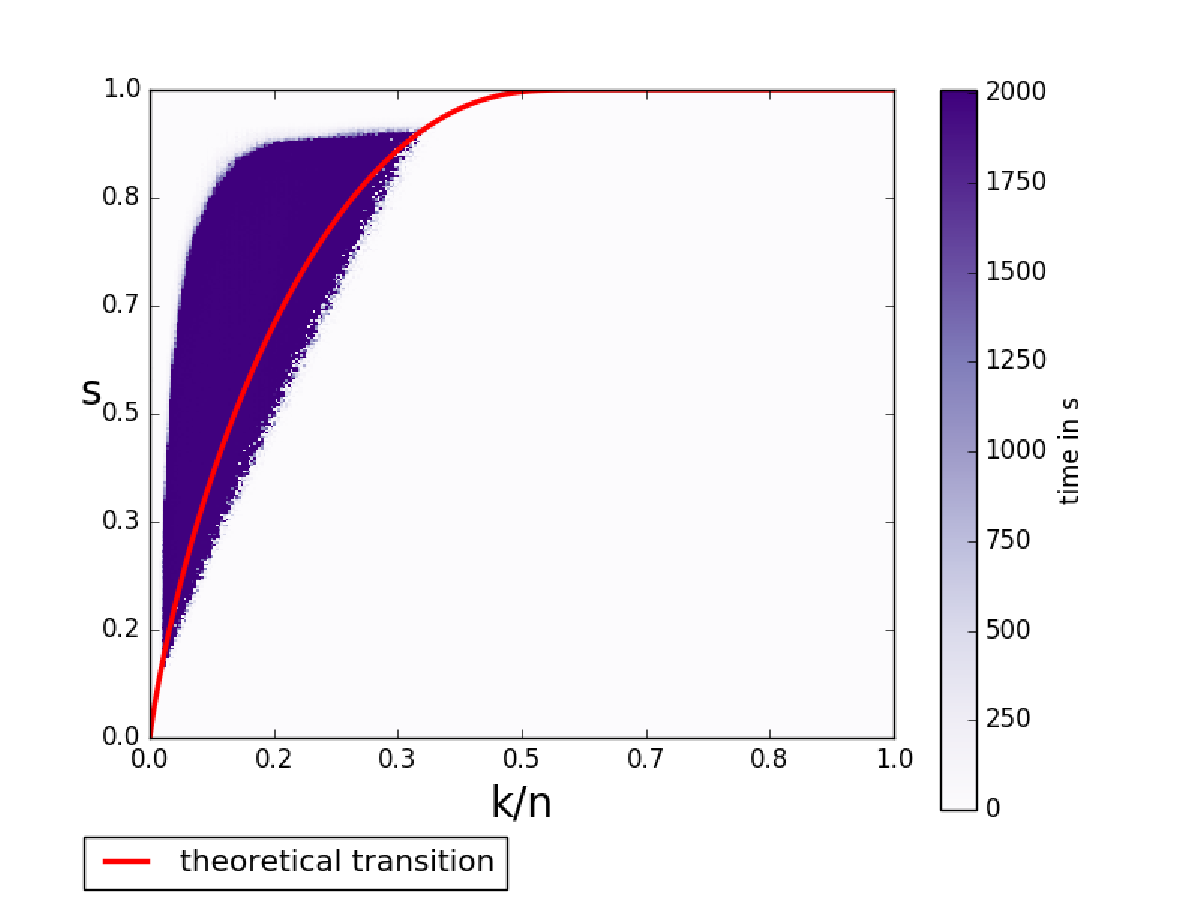
\includegraphics[width=1\linewidth]{pb-experiments/runtime/card/300_runtime.pdf}\par
		\captionof{figure}*{$n=300$}
	\end{multicols}
	\caption{Three plots for $\cardnet$ encoding. Each plot shows the runtime behavior for a different number of variables in the following order: (a) $n=100$ , (b) $n=200$, and (c) $n=300$. The purple region is where the blowup in runtime was observed. The red line indicates the phase transition. (Best viewed in color) \label{fig:ncomp}}
\end{figure*}
\section{Experimental Results} \label{sec:experiments}
\subsubsection{Experimental Setup}
\blfootnote{The data and scripts associated with this project are available at \url{https://github.com/meelgroup/1-CARD-XOR} } \label{sec:experiments:scaling:setup}
For every value of $n$, $k$ and $s$ we generate $\FQ$ in the following manner. To uniformly choose an XOR-clause, we include each variable of $\{x_1,\cdots,x_n\}$ with probability $\frac{1}{2}$ in the XOR clause. We then choose exactly one of $\{0,1\}$ with probability $\frac{1}{2}$ in the XOR clause. We repeat such uniform sampling of XOR clauses $\ceil{sn}$ many times and conjunct all such XOR-clauses to build $\Q$. Finally, we conjuct $\Q$ with $\F$ to generate $\FQ$. 

We performed experiments with $9$ values of $n$. For each $n\in \{ 50,75,100,125,150,175,200,250,300\}$ we generated an instance of 1-CARD-XOR for all values of $k \in [0,n]$ and $\ceil{sn} \in [1,n]$. We repeated the experiments 10 times for each data point with $n=\{75,100\}$ to get a finer estimate on the satisfiability at the transition threshold. We were not able to run experiments for values of $n$ significantly larger than those listed above due to computational constraints.

Since \CryptoMiniSAT~\cite{SNC09} is a specialized solver which handles XOR clauses in combination with CNF clauses quite efficiently, we use it as the SAT solver in our experiments. We used a high performance computing cluster of 25 nodes for our experiments. Each node consisted of an Intel\textsuperscript{\textregistered} Xeon\textsuperscript{\textregistered} E5-2690 v3 CPU with 24 cores and 96GB of RAM divided evenly among the cores, with each core having access to 4GB of RAM. Each experiment was conducted on a single core. Our experimental evaluation used over 80,000 CPU hours. 

It is known that encoding cardinality constraint using different encodings may result not only in different sizes for $\F$ but also may have an impact on the performance of the solver.
To investigate the impact of various encodings of cardinality constraints for 1-CARD-XOR formulas, for each value of $n$, $s$ and $k$ we experimented with three cardinality encodings.
  \begin{itemize}[itemsep=1pt]
	\item Adder: $\bigO(n)$ clauses, no arc consistency ~\cite{ES06}
	\item BDD:   $\bigO(n\cdot k)$ clauses, preserves arc-consistency, is equivalent to $LT^{n,k}_{SEQ}$ encoding ~\cite{Sinz05} 
	\item Cardinality Network:  $\bigO(n\cdot log^2 k)$ clauses, preserves arc consistency ~\cite{CardinalityNA09} 
\end{itemize} 
In our experiments, we have used the PBLib ~\cite{pblib} tool to encode our constraints.
A timeout of $2000$ seconds was used for all experiments. 
\subsubsection{Polarity Caching}
The SAT solver goes through an iterative process of search and inference. During search, it selects an unassigned variable and then decides on the truth value (polarity) to be given to this variable.
During inference phase it explores the implications of these choices until we either get a contradiction or a satisfying assignment or nothing further can be inferred and the solver has to  make another variable selection. Polarity selection heuristics decide which truth value, either {\tt true} or {\tt false} to assign to the selected variable. When the solver backtracks due to a contradiction, it must explore  the other choice for the truth value. A heuristic which works very well in practice is polarity caching \cite{DBLP:conf/sat/PipatsrisawatD07}, which involves remembering the previous successful choice made on a particular variable. Another simpler heuristic is setting the polarity to {\tt false}, which instructs the solver to always explore the {\tt false} branch before the {\tt true}. As discussed later, setting the polarity to {\tt false} always significantly improves the runtime performance of the solver. Therefore, the experiments concerning runtime performance of SAT solver with respect to other parameters were performed with setting polarity flag to {\tt false} in \CryptoMiniSAT. 




%This is evident in Figure \ref{fig:caching} where we see the difference in performance.

\paragraph{Results}
The objective of our experimental evaluation is to answer these four research questions:
\begin{enumerate}[itemsep=1pt,leftmargin=9.5mm]
	\item[\bf{RQ1.}] How does the satisfiability of $\FQ$ vary, as parameters $k$  and XOR clause density $s$ vary ?
	\item[\bf{RQ2.}] How does the runtime performance of SAT solver for $\FQ$ vary with respect to $n$, $k$, $s$?
	\item[\bf{RQ3.}] How do the different encodings affect the runtime performance of the SAT solver for $\FQ$?
	\item[\bf{RQ4.}] How do the different branching heuristics affect the runtime performance of a SAT solver on $\FQ$?
\end{enumerate}
We now first present detailed analysis below and then summarize our main conclusions. 

\paragraph{\bf{RQ1.}}Figure~\ref{fig:satisfiablitiy} shows the satisfiability of random instances of $\FQ$ as the density of XOR-clauses $s$  and the upper bound on at-most-k constraint $k$ varies. The y-axis indicates the density $s$ and the x-axis indicates $k/n$. Each point on the plot is color-coded to represent satisfiability of the corresponding $\FQ$. The dark blue color indicates that the corresponding formula is satisfiable while light color indicates unsatisfiability. The red curve represents the theoretical phase transition curve,  obtained in Section \ref{sec:analysis}, i.e., a point in the region under the curve is likely to be satisfiable while a point in the region over the curve is likely to be unsatisfiable. We observe that the empirically observed behavior agrees with the analysis, thus demonstrating the tightness of our analysis. 

\begin{figure*}
	\begin{multicols}{3}
		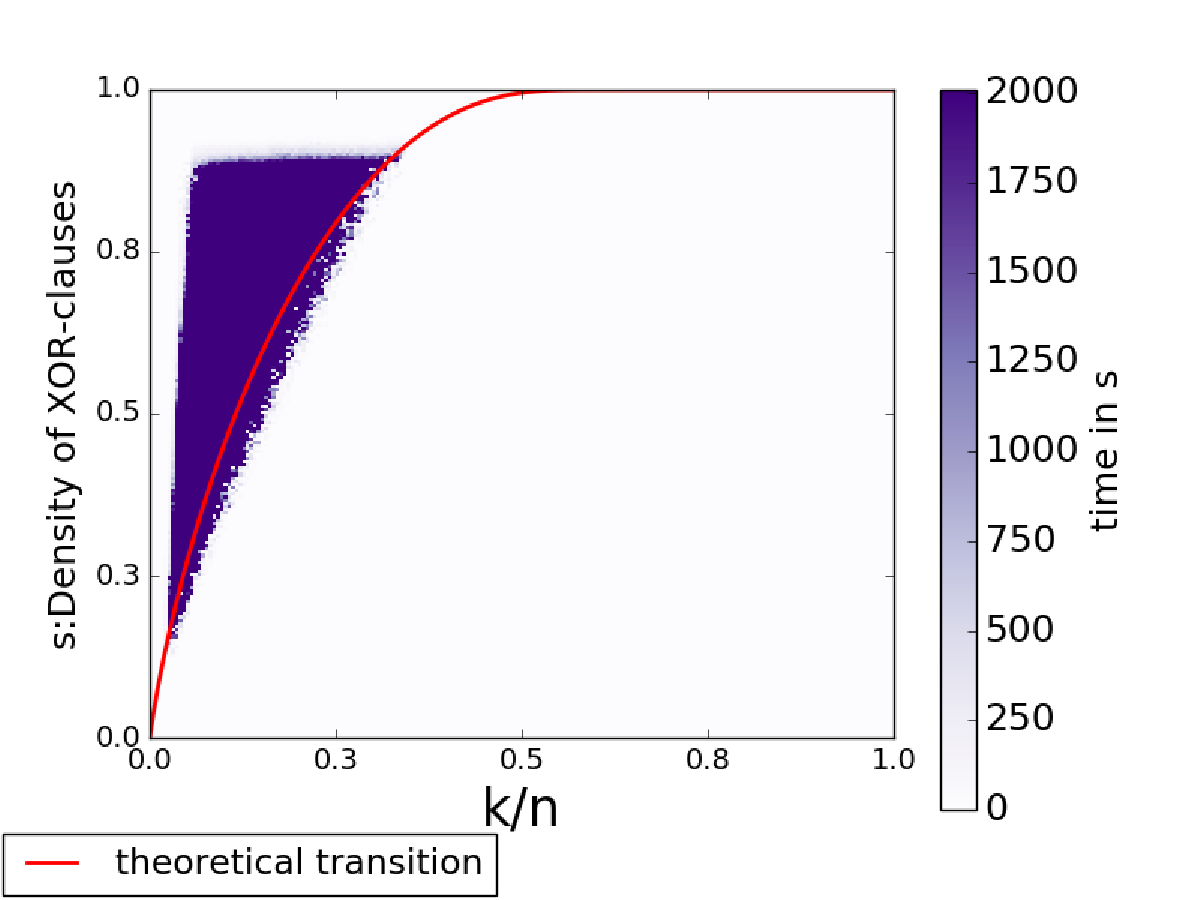
\includegraphics[width=1\linewidth]{pb-experiments/runtime/adder/200.pdf}\par
		\captionof{figure}*{\adder}
		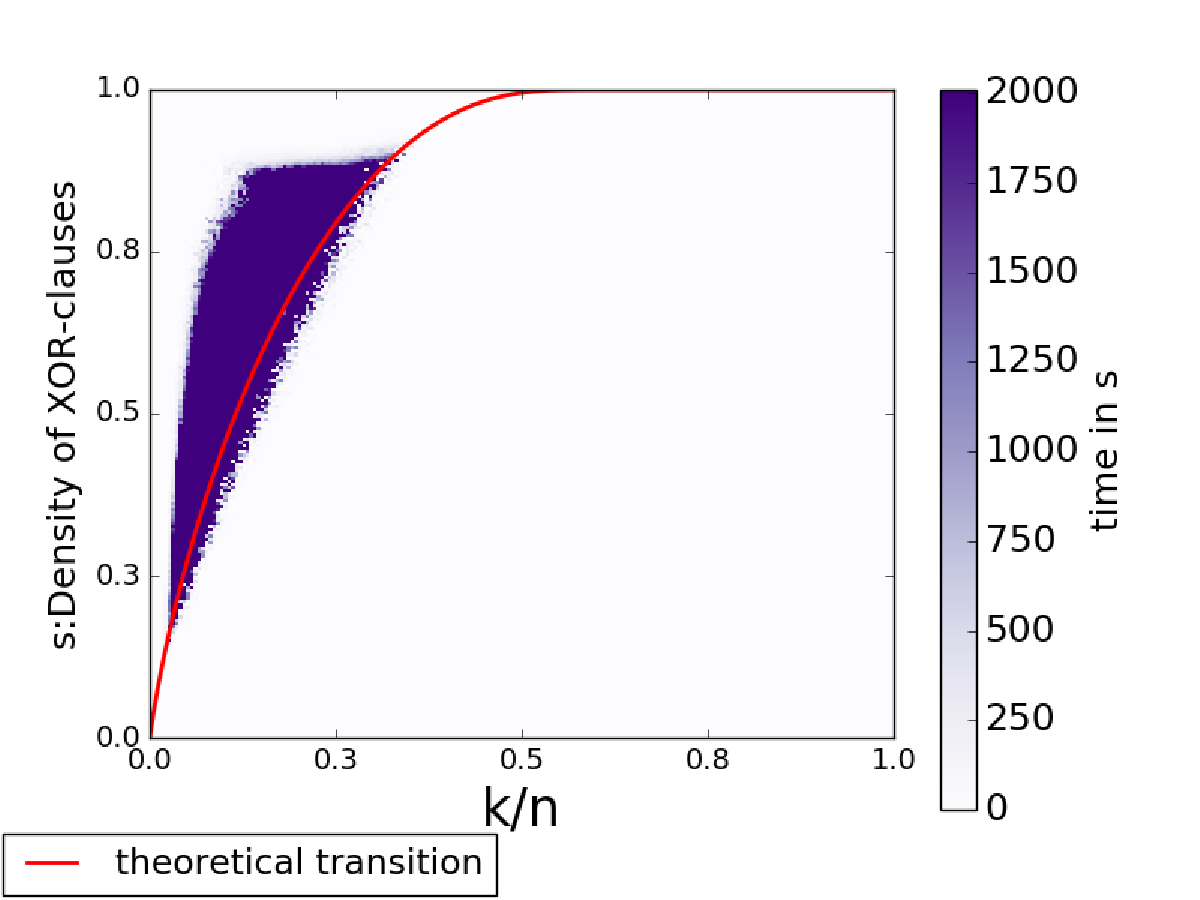
\includegraphics[width=1\linewidth]{pb-experiments/runtime/bdd/200.pdf}\par 
		\captionof{figure}*{\bdd}
		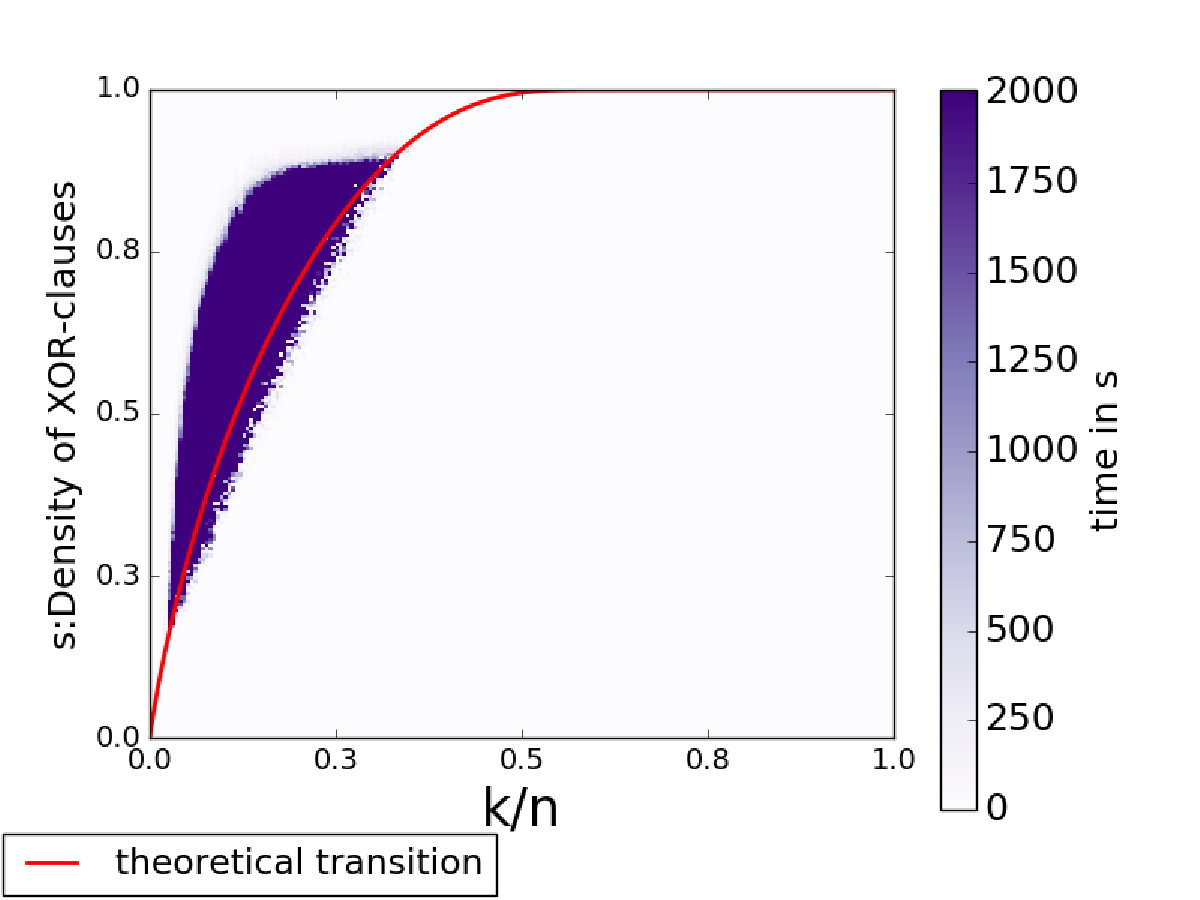
\includegraphics[width=1\linewidth]{pb-experiments/runtime/card/200.pdf}\par
		\captionof{figure}*{\cardnet}
	\end{multicols}
	\caption{Three plots for $n=200$. Each plot shows the runtime behavior for a different encoding in the following order: (a) \adder, (b) \bdd, and (c) \cardnet. The purple region is where the blowup in runtime was observed. The red line indicates the phase transition.\label{fig:enccomp}}
\end{figure*}

\begin{figure}
	\begin{multicols}{2}
		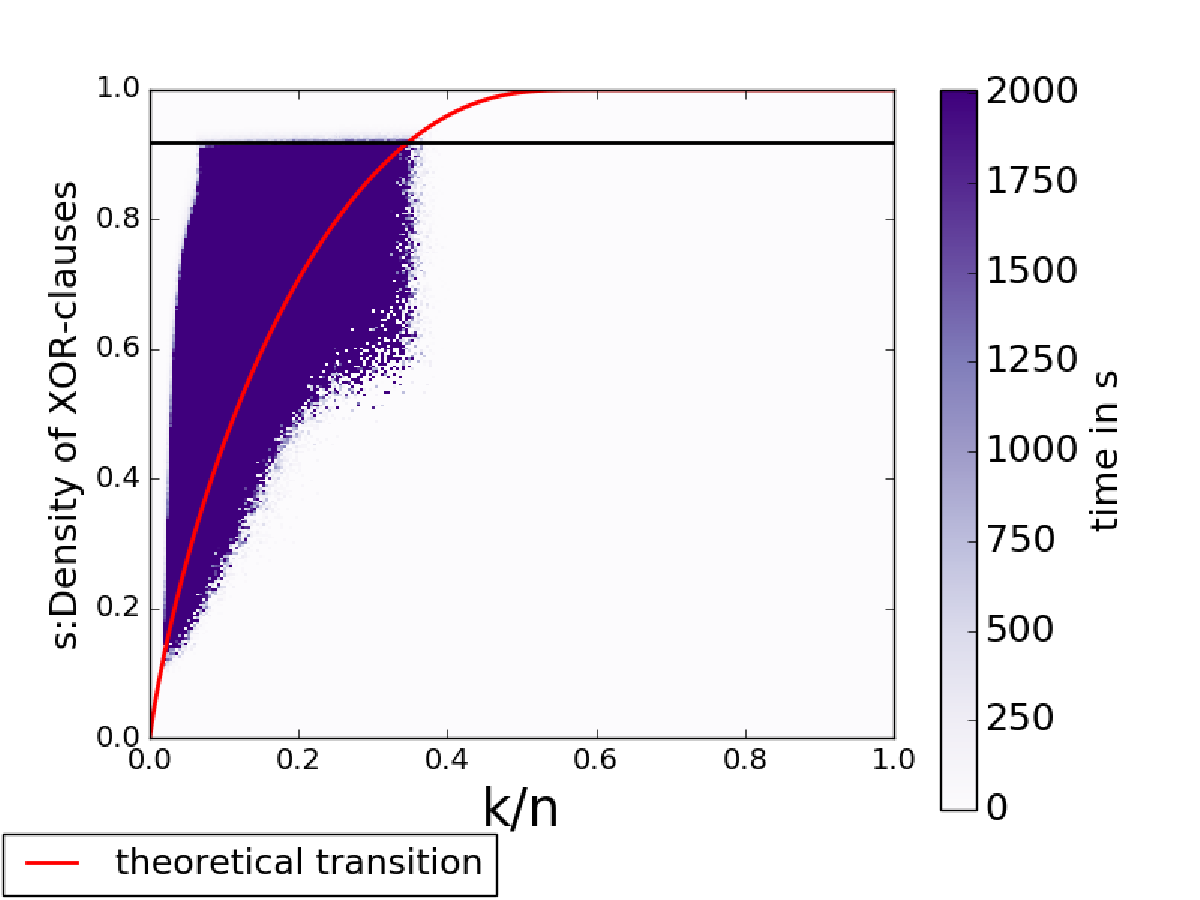
\includegraphics[width=\linewidth,height=\linewidth]{pb-experiments/polarity-false/adder/250.pdf}\par
		\captionof{figure}*{(a)}
		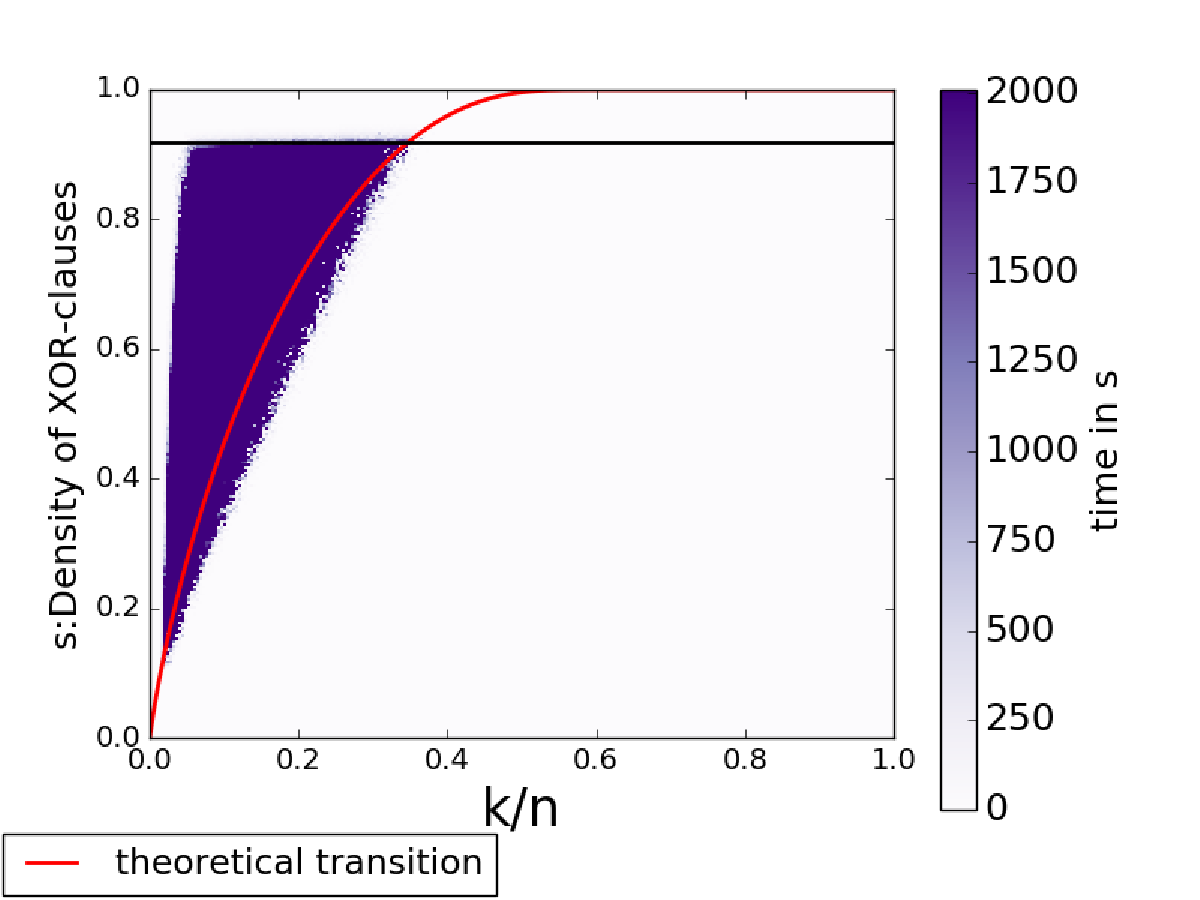
\includegraphics[width=\linewidth,height=\linewidth]{pb-experiments/polarity-false/adder/250_false.pdf}\par
		\captionof{figure}*{(b)}
	\end{multicols}
	\captionof{figure}{$n=250$, \adder. The purple region shows the hard instances for the solver when (a) polarity caching was used and (b)when the solver was made to explore the \false branch first.}	\label{fig:caching} 
\end{figure}

\paragraph{\bf{RQ2.}}We now turn our attention to a study of scaling behavior of runtime performance of SAT solver. Figure~\ref{fig:ncomp} shows the runtime performance for increasing values of $n$, i.e., $n \in \{100,200,300\}$. Similar to Figure~\ref{fig:satisfiablitiy}, the x-axis indicates  $k/n$ while the y-axis indicates the density $s$. Note that most of the instances were solvable in just 2 seconds but the instances within the purple region timed out for timeout of 2000 seconds. Furthermore, we observe that the area of {\em hard} instances increases with $n$. The sudden increase in runtime around the phase transition is reminiscent of similar behavior for random CNF instances but is unlike the behavior observed in case of CNF-XOR formulas~\cite{DMV17}. This behavior necessitates further research for a deeper understanding, and we hope this deeper understanding would be useful in the design of efficient CARD-XOR solvers.  
\paragraph{\bf{RQ3.}}Given the widespread interest in the design of different encodings for CARD constraints, it is natural to ask whether the runtime behavior of $\FQ$ is sensitive to encodings. To this end, Figure~\ref{fig:enccomp} shows the runtime performance of SAT solvers for the above mentioned three different encodings: \adder, \bdd, and \cardnet. Similar to Figure~\ref{fig:satisfiablitiy}, the x-axis indicates  $k/n$ while the y-axis indicates the density $s$. We observe that while the area of the purple region deviates slightly across for different encodings, the qualitative behavior around phase transition regions very similar. 





 \paragraph{\bf{RQ4.}} We now turn to the question, what effect do the branching heuristics have on the runtime behavior of SAT solver for $\FQ$. Figure~\ref{fig:caching}(a) shows the behavior when polarity caching was used while Figure~\ref{fig:caching}(b) shows the behavior when the solver always set the {\tt polarity} flag to {\tt false}. The value of $n$ is set to 200 for both the cases. Interestingly, we observe a significant reduction in the area of the purple region by always setting {\tt polarity} flag to {\tt false}, which is surprising given polarity caching has shown to achieve significant gains for SAT solving. A detailed study of different heuristics is beyond the scope of this work and is left for future work.

